\documentclass[pdf, 10pt, koi8-r]{beamer} %Для Latex2Pdf  tex -> pdf
%В качестве размера лучше использовать 9pt
%dvips нужно использовать только если использовать построение слайдов через PostScript
%intlimits - стиль для пределов интегралов (по желанию)
%unicode - обязательно

%Пакеты для русского языка
\usepackage[T2A]{fontenc}
\usepackage[utf8]{inputenc}
\usepackage[english,russian]{babel}
\usepackage{indentfirst}

\usepackage{graphicx}
%\usepackage[font=small]{caption,subfig}
\usepackage{times}
\usepackage{cmap}
\usepackage{mathptmx}

\usepackage{amsmath}
\usepackage{amsfonts}
\usepackage{amsbsy}
\usepackage{amssymb}
\usepackage{amsthm}

\usetheme{Montpellier}
\usepackage{hhline}
\usepackage{longtable}
\usefonttheme[onlymath]{serif}

\setbeamertemplate{headline}{%
\begin{beamercolorbox}{section in head/foot}
{\ }\hfill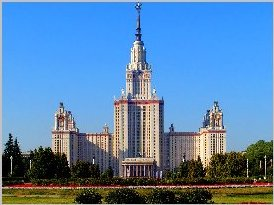
\includegraphics[scale=0.08]{pics/msu.jpg}\hskip2pt{\ }\vskip-21pt
\end{beamercolorbox}%
}

% Сюда вствить ФИО и номер группы
\def\FullName{Нагорных Яна Валерьевна}
\def\ShortName{Нагорных Я.В.}
\def\Group{410}
%\def\PaperType{Дипломная работа}
\def\PaperType{Курсовая работа}


\setbeamertemplate{footline}{%
\begin{beamercolorbox}{section in head/foot}
\vskip1pt{\ }\hskip1pt%
\ShortName\hfill{}\PaperType%
\hskip1pt{\ }\vskip1pt%
\end{beamercolorbox}%
}


% Удаляем навигационную панель
\setbeamertemplate{navigation symbols}{}

% Устанавливаем поля (по умолчнанию - 1 см)
\setbeamersize{text margin left=0.5cm, text margin right=0.25cm}

%Более крупный шрифт для подзаголовков титульного листа
\setbeamerfont{institute}{size=\normalsize}

%Задание команды (\bluetext) для выделения конкретным (синим) цветом
%\alert - выделение цветом выбранной "темы"
\setbeamercolor{bluetext_color}{fg=blue}
\newcommand{\bluetext}[1]{{\usebeamercolor[fg]{bluetext_color}#1}}

\setbeamercovered{transparent}

% Путь к файлам с иллюстрациями
\graphicspath{{img/}}

\def\MyColorBox#1{{%
\centering
\textcolor{blue}{%
\fbox{\textcolor{black}{%
\parbox{0.98\textwidth}{\centering\parbox{0.97\textwidth}{%
\noindent\strut{}%
#1\strut}}}}}%
}}


\title{Реализация библиотеки параллельной записи больших файлов с вещественными числами в текстовом представлении}

\author[\FullName]{\FullName \newline студент \Group{} группы}

 \institute{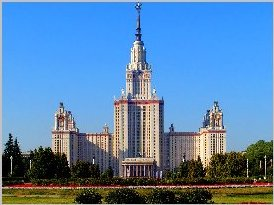
\includegraphics[scale=0.3]{./pics/msu.jpg} \\[2ex] 
  Научный руководитель --- д.\,ф.-м.\,н., доцент \,{К.Ю. Богачев }\\ }
  \date{     Москва,     2018г. }

\newcommand{\col}{\textcolor[rgb]{0.2,0.2,0.75}}
\renewcommand{\figurename}{Рисунок}
\begin{document}
\frame{
\titlepage
}

\frame{
\frametitle{Введение}
Печать больших массивов чисел без округления с большой точностью всегда занимает много времени.
Однако, не вся печать упирается в возможности диска, как это может показаться.
Кроме того, у печати данных мало ресурсов для ускорения.\\
\vspace{14pt}
\textbf{\col{Цели работы:}}
\begin{enumerate}
\item Ускорить печать больших массивов без потери точности;
\item Использовать быстрые алгоритмы печати целых чисел и чисел с плавающей точкой.
\end{enumerate}
\vspace{14pt}
\textbf{\col{Возможные варианты улучшений}}
\begin{itemize}
\item Применение более быстрых алгоритмов преобразования чисел в строки
\item Использование многопоточного программирования
\item Изменение формата вывода (отбрасывание лишних нулей, сокращенная запись повторяющихся чисел)
\end{itemize}
}

\section{Описание алгоритма}
\frame{
\frametitle{Описание алгоритма}
\col{Распределение задач}
\begin{figure}[h!]
\begin{tiny}
\def\svgwidth{300pt}
  \input{pics/drawing.pdf_tex}
\end{tiny}
\end{figure}
\begin{center}
\footnotesize{\col{Рисунок 1.} Работа потоков}
\end{center}
}
\frame{
\col{Алгоритм Grisu}
\begin{itemize}
\item Выражаем $v$: $$v=\cfrac{f_v}{2^{-e_v}}.$$
\item Десятичные цифры $v$ могут быть вычислены путем нахождения десятичного показателя $t$, для которого $$1 \leqslant \cfrac{f_v \times 10^t}{2^{-e_v}} < 10.$$
\item Идея \textsf{Grisu} состоит в кэшировании значений дробей $\cfrac{10^t}{2^{e_t}}$.
\end{itemize}
\vspace{10pt}
\col{Алгоритм Grisu2}
\begin{itemize}
\item У \textsf{Grisu} есть существенный недостаток: все числа выводятся в экспонециальном виде.
\item В отличие от \textsf{Grisu} алгоритм \textsf{Grisu2} не генерирует полное десятичное представление, а просто возвращает значащие цифры и соответствующий показатель. 
Затем процедура форматирования объединяет эти данные для получения представления.
\end{itemize}
}
\frame{
\frametitle{Пример работы Grisu2}
\begin{figure}[h!]
\begin{center}
\begin{tabular}{|l|c|l|}
\hhline{|-|~|-|}
  array[0] = 1;				& & 1 \\
  array[1] = 1.2;			& & 1.2 \\
  array[2] = 1.23;			& & 1.23\\
  array[3] = 1.23400000;	& & 1.234 \\
  array[4] = 1.23456789;	& & 1.23456789\\
  array[5] = -1;			& & -1\\
  array[6] = -1.234;		& $\longrightarrow$ & -1.234\\
  array[7] = sqrt (2);		& & 1.4142135623730952\\
  array[8] = 1234e-36;		& & 1.234e-33\\
  array[9] = 0.000000123;	& & 1.23e-7\\
  array[10] = 0.123;		& & 0.123\\
  array[11] = 12.3;			& & 12.3\\
  array[12] = 123.000;		& & 123\\
  array[13] = 1.234e2;		& & 12.34\\
\hhline{|-|~|-|}
\end{tabular}
\textit{ 
\begin{tabular}{ccc}
$\quad\qquad$ массив $\qquad\qquad$ & $\quad\quad$ & выходной файл \\
\end{tabular}\\
}
\vspace{14pt}
\footnotesize{\col{Рисунок 2.} Полученный с помощью Grisu2, выходной файл для данного массива.}
\end{center}
\end{figure}
}

\frame
{
\frametitle{Результаты работы}
\col{Случайные числа.} Среднее время работы в секундах:
\begin{small}
\begin{center}
\begin{tabular}{||c|c|c|c|c|c|c||}
\hline
\hline
Размер & \multicolumn{4}{c|}{Число потоков} & Стандартная & Размер\\
\hhline{~|-|-|-|-|~|~|}
массива & 6 & 4 & 2 & 1 & печать &файла\\
\hline
\hline
$10^7$   & 0.562 & 0.841 & 1.578 & 3.162 & 4.207 & 245 MB \\
\hline
$5 \cdot 10^7$  & 3.013 & 4.223 & 8.070 & 15.91 & 21.79 &  1.2 GB\\
\hline
$10^8$  & 5.167 & 8.112 & 15.45 & 31.24 & 41.86 & 2.4 GB\\
\hline
$5 \cdot 10^8$ & 40.80 & 49.35 & 75.31 & 148.39 & 200.33 & 12 GB\\
\hline
\hline
\end{tabular}
\end{center}
\end{small}
Среднее ускорение работы алгоритма приведено в таблице далее. 
Ускорение на одном потоке демонстрирует ускорение работы \textsf{Grisu2} по сравнению со стандартной печатью.
\begin{small}
\begin{center}
\begin{tabular}{||c|c|c|c|c||}
\hline
\hline
Размер & \multicolumn{4}{c||}{Число потоков}\\
\hhline{~|-|-|-|-|}
массива & 6 & 4 & 2 & 1 \\
\hline
$10^7$ &  7.49  & 5.00 & 2.67 & 1.33 \\
\hline
$5 \cdot 10^7$ & 7.23 & 5.16 & 2.70 & 1.37 \\
\hline
$10^8$ & 8.10 & 5.16 & 2.71 & 1.34\\
\hline
$5 \cdot 10^8$ & 4.91 & 4.06 & 2.66 & 1.35\\
\hline
\hline
\end{tabular}
\end{center}
\end{small}
}
\frame{
Наглядно зависимость времени от числа потоков для массива размером $10^8$ изображена на графиках.
\begin{figure}[h!]
\begin{minipage}[h]{0.45\linewidth}
\center{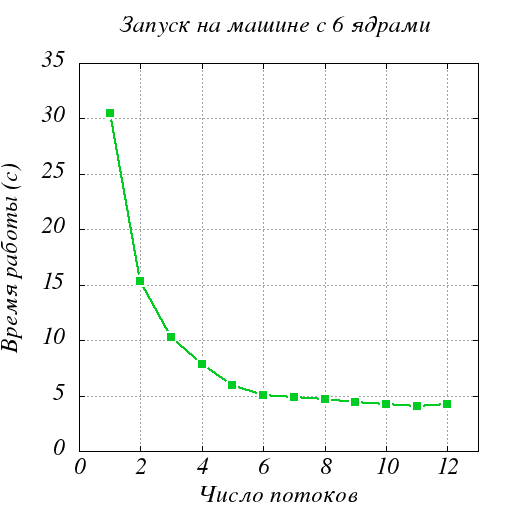
\includegraphics[width=1\linewidth]{./pics/time.png}}
\end{minipage}
\hspace{5pt}
\begin{minipage}[h]{0.45\linewidth}
\center{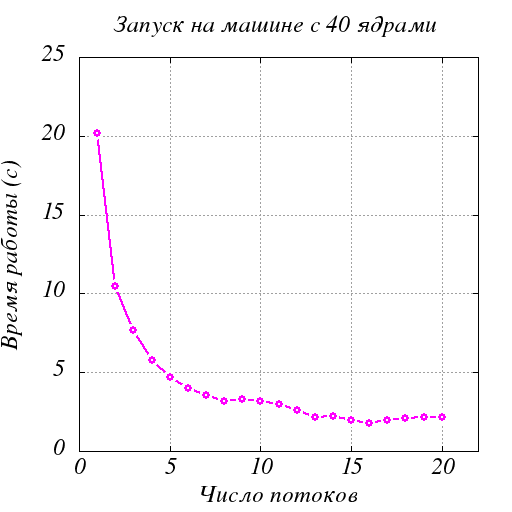
\includegraphics[width=1\linewidth]{./pics/time40.png}}
\end{minipage} 
\end{figure}
\begin{center}
\footnotesize{\col{Рисунок 3.} Зависимость времени работы от числа потоков.}
\end{center}
}
\frame{
\col{Целые числа}
\begin{small}
\begin{center}
\begin{tabular}{||c|c|c|c|c|c|c||}
\hline
\hline
Размер & \multicolumn{4}{c|}{Число потоков} & Станд. & Размер\\
\hhline{~|-|-|-|-|~|~|}
массива & 6  & 4 & 2 & 1 & печать & файла\\
\hline
\hline
$10^7$ & 0.301 & 0.352 & 0.695 & 1.400 & 5.686  &56 MB / 205 MB \\
\hline
$5 \cdot 10^7$& 1.381  & 1.674 & 3.344 & 6.443 & 29.06  &295 MB / 1 GB\\
\hline
$10^8$ & 2.424 & 3.330 & 6.628 & 12.95 & 55.54  & 590 MB / 2 GB \\
\hline
$5 \cdot 10^8$ & 11.92 & 16.57 & 32.11 & 63.57 & 286.70  &2.9 GB / 10 GB\\
\hline
\hline
\end{tabular}
\end{center}
\end{small}
Размер файла, полученного с помощью нового алгоритма гораздо меньше размера файла, полученного стандартной печатью, так как отброшены лишние нули.
За счет этого ускорение возросло:
\begin{small}
\begin{center}
\begin{tabular}{||c|c|c|c|c||}
\hline
\hline
Размер & \multicolumn{4}{c|}{Число потоков}\\
\hhline{~|-|-|-|-|}
массива & 6 & 4 & 2 & 1 \\
\hline
$10^7$  & 18.87 & 16.19 & 8.17 & 4.06 \\
\hline
$5 \cdot 10^7$ & 21.04 & 17.36& 8.69 & 4.51 \\
\hline
$10^8$ & 22.91 & 16.82 & 8.38 & 4.29 \\
\hline
$5 \cdot 10^8$ & 24.03  & 17.30 & 8.93& 4.51 \\
\hline
\hline
\end{tabular}
\end{center}
\end{small}
}
\frame{
\col{Повторяющиеся числа}
\begin{small}
\begin{center}
\begin{tabular}{||c|c|c|c|c|c|c||}
\hline
\hline
Размер & \multicolumn{4}{c|}{Число потоков} & Станд. & Размер \\
\hhline{~|-|-|-|-|~|~|}
массива & 6 & 4 & 2 & 1 & печать  & файла\\
\hline
\hline
$10^7$ & 0.114 & 0.169 & 0.328 & 0.643 & 3.422  & 24 MB / 187 MB \\
\hline
$5 \cdot 10^7$ & 0.535 & 0.840 & 1.633 & 2.97 & 17.10  & 123 MB / 936 MB\\
\hline
$10^8$ & 1.164 & 1.704 & 3.280 & 6.022 & 36.31  & 245 MB / 1.8 GB\\
\hline
$5 \cdot 10^8$ &5.748 & 8.368 & 16.23 & 31.46 & 182.50  & 1.2 GB / 9.4 GB\\
\hline
\hline
\end{tabular}
\end{center}
\end{small}
За счет того, что все последовательности одинаковых подряд идущих чисел будут сворачиваться в короткую строку вида \texttt{n*x}, уменьшился файл и увеличилось ускорение.
\begin{small}
\begin{center}
\begin{tabular}{||c|c|c|c|c||}
\hline
\hline
Размер & \multicolumn{4}{c|}{Число потоков}\\
\hhline{~|-|-|-|-|}
массива & 6 & 4 & 2& 1 \\
\hline
$10^7$  & 30.08 & 20.13 & 10.46 & 5.33 \\
\hline
$5 \cdot 10^7$ & 31.98 & 20.32 & 10.47 & 5.74 \\
\hline
$10^8$ & 31.20 & 21.31 & 11.07 & 6.03 \\
\hline
$5 \cdot 10^8$ & 31.75 & 21.81 & 11.54 & 5.80 \\
\hline
\hline
\end{tabular}
\end{center}
\end{small}
}
\frame{
\col{Огромные массивы случайных чисел}\\
\begin{minipage}[h]{140pt}\begin{itemize}
\item Сравним стандартную печать и алгоритм, запущенный на 12 (+2) потоках.
\item Помимо обычного запуска, проведем и запуск с записью не на диск, а в разделяемую память \textit{shared-memory}.
\item На следующем графике приведена зависимость времени работы от размера массива.
\end{itemize}
\end{minipage}
\begin{minipage}[h]{180pt}
\vspace{5pt}
\begin{figure}[h!]
\center{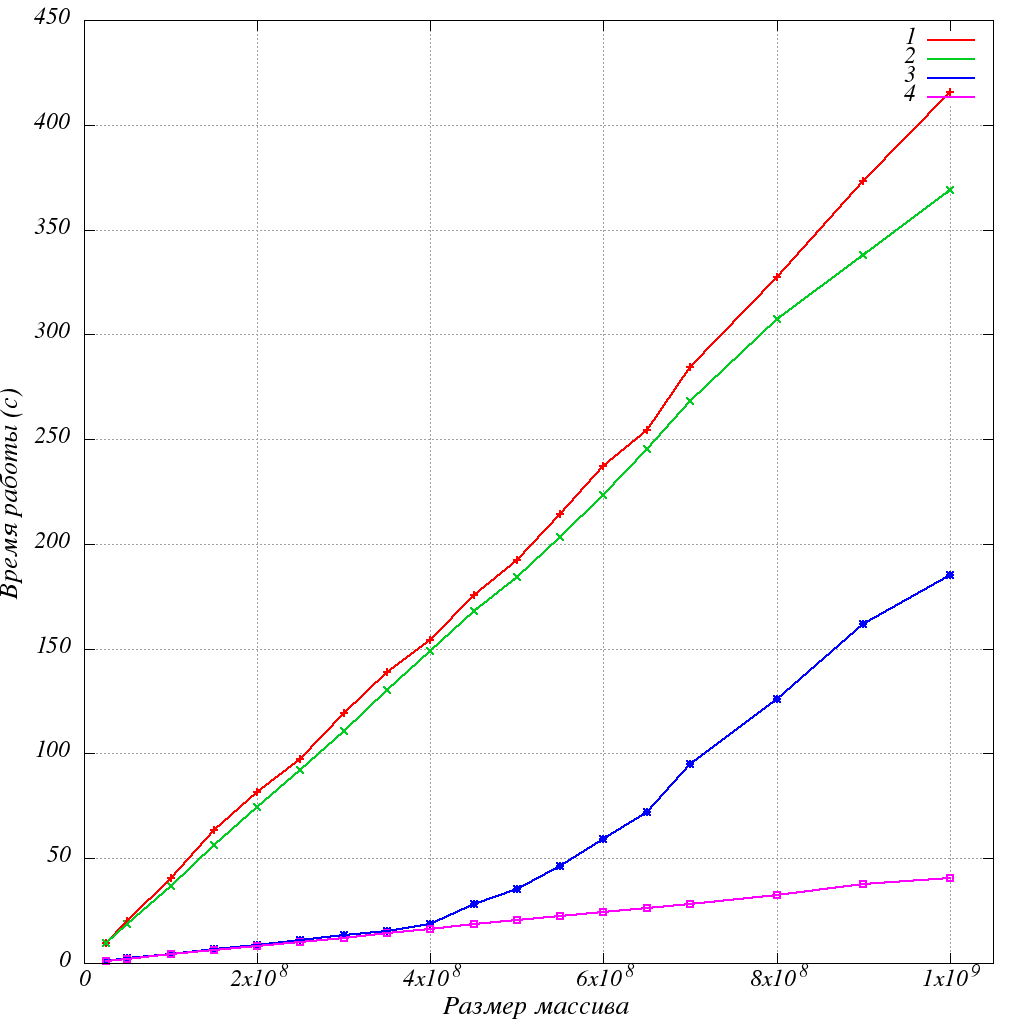
\includegraphics[width=180pt]{./pics/graphics.png}}
\end{figure}
\tiny {1 -- стандартная печать с записью на диск;
2 -- стандартная печать с записью в разделяемую память;  3 -- алгоритм параллельной печати с записью на диск; 4 -- алгоритм параллельной печати с записью в разделяемую память.}
\end{minipage}
}
\frame{
\frametitle{Заключение}
\begin{itemize}
\item В результате написания курсовой работы была решена поставленная задача: 
реализована библиотека параллельной записи массивов вещественных чисел.
\vspace{14pt}
\item В ходе тестирования была проверена точность работы реализованного алгоритма, а также измерено ускорение в сравнении со стандартной функцией печати. 
\vspace{14pt}
\item Написанная на языке \textsf{С++} подпрограмма была внедрена в промышленный гидродинамический симулятор \textsf{tNavigator}.
\end{itemize}
}
\frame{
\begin{center}
\Huge{\col{Спасибо за внимание!}}
\end{center}
}
\frame{
\frametitle{Список использованной литературы}
\begin{thebibliography}{}
\bibitem{1} \textsc{Florian Loitsch}.
Printing Floating-Point Numbers Quickly and Accurately with Integers, 2004.
\vspace{14pt}
\bibitem{2} \textsc{Wojciech Mu\l a}.
SSE: conversion integers to decimal representation, 2011.
\vspace{14pt}
\bibitem{3} \textsc{Богачев К.Ю.}.
Основы параллельного программирования. -- M.: Бином. Лаборатория знаний, 2010.
\vspace{14pt}
\bibitem{4} \textsc{David Goldberg.}
What every computer scientist should
know about floating-point arithmetic. -- ACM Computing Surveys, 23(1): 5–48, 1991.
\end{thebibliography}
}
\end{document}